\chapter{Possible realizations of an EIC} 
\label{chp:EIC}

\section{The designing requirement of a future EIC}
The EIC is a multi-purpose collider designed to answer a wide range
of the most compelling science questions concerning to our fundamental understanding of QCD physics. The most intriguing questions
that an EIC will address include:
\begin{itemize}
\item The spin distribution in space and momentum for sea quarks and gluons inside the nucleon.
\item The impact of the nuclear environment cast on the distribution of quarks and gluons and their interactions in nuclei.
\item The collective gluon dynamics in the saturation regime.
\end{itemize}
Two independent designs for the realization of a future EIC have been developed
in the United States. At the Brookhaven National Laboratory (BNL), the eRHIC
design is planning to build a new electron beam inside the RHIC tunnel to
collide with the currently existing polarized proton and nuclear beams at RHIC.
On the other hand, at the Thomas Jefferson National Laboratory (JLab), the MEIC
design utilizes a new electron and ion collider ring complex together with the
recently upgraded 12 GeV CEBAF accelerator at JLab.

The targeted physics programs put some requirements on the EIC machine designs.
To deliver enough physics statistics in a promising time, a high luminosity
$\sim 10^{33} \mathrm{cm}^{-2}\mathrm{s}^{-1}$ is required. Extracting the
structure function and exploring the nuclear time-space evolution needs flexible beam
energy in a wide range. To study the spin distribution, electrons and proton/light
nuclei must be highly polarized. A large variety of nuclear beams are needed to study
the nuclear size dependence. In the semi-inclusive DIS studies, a wide acceptance
detector with good particle identification (PID) is inevitable. For some exclusive
measurements, it is demanding to have the acceptance for protons generated in the
very forward region.

Although the two realizations from BNL and JLab have similar collision parameters,
depending the specific upgrade plan, some differences still exist. For the following
discussions, I will focus on the eRHIC design of the EIC. 


\section{The eRHIC design possibilities}

\subsection{The eRHIC collider parameters}
A cost-effective way of building a full-energy EIC from day one using and an
Energy Recovery LINAC (ERL) with a Fixed-Field Gradient-Accelerator (FFAG)
design is found at BNL as shown in Fig.~\ref{fig:collider_eRHIC}.
\begin{figure}
\centering
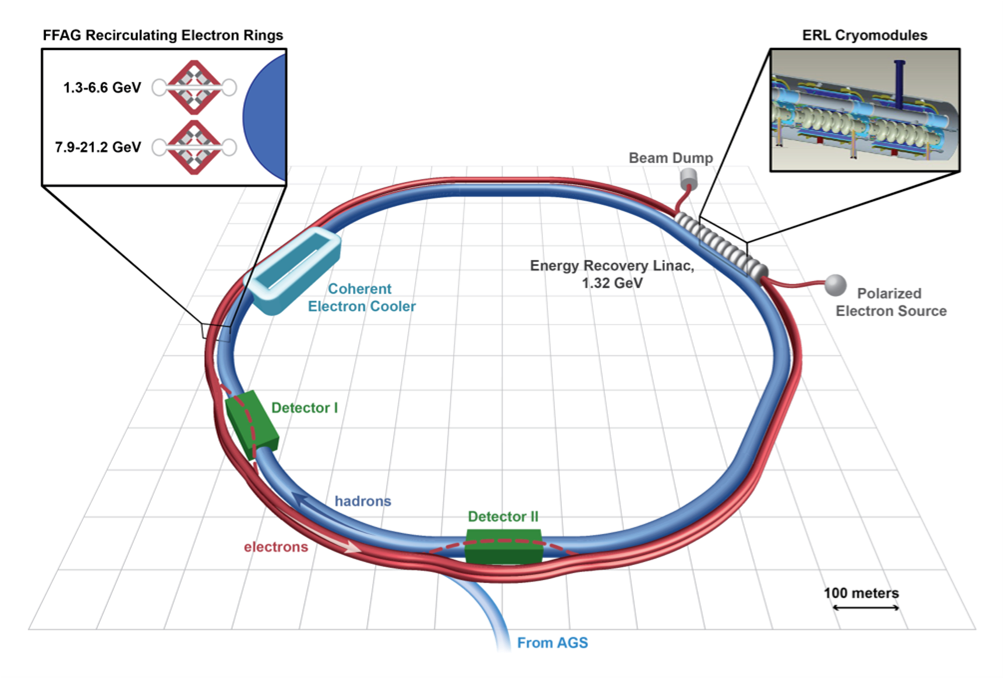
\includegraphics[width=0.9\textwidth]{plots/chpt4/collider_eRHIC.png}
\caption[eRHIC collider design]{
The collider design for eRHIC. The plot is from BNL-CAD eRHIC group.}
\label{fig:collider_eRHIC}
\end{figure}
The current eRHIC machine design allows us to have an electron beam at the
energy ranging from 5 GeV to 21.2 GeV with the beam polarization up to 80\%.
Meanwhile, the existing RHIC facility is capable of providing a proton beam with
70\% polarization at 100-250 GeV. Unpolarized light ions (e.g. dueterium,
silicon) and heavy ions (gold, uranium) are also available to be accelerated to
50-100 GeV/nucleon. There is also the possibility to accelerate the polarized
light ions ($He^{3}$) up to an energy of 167 GeV/nucleon. The full range of
proton/ion beam energies will be accessible from the beginning of operations,
while the electron beam energy will start with 10-15 GeV and later be increased
to 20 GeV. As a result, the available beam energies altogether provide an
accessible center of mass energy range 30-145 GeV.



\subsection{An eRHIC model detector}
To fulfill the requirements on the detector postulated by different physics processes, a generic model detector design has been developed and shown in Fig.~\ref{fig:detector_eRHIC}.
\begin{figure}
\centering
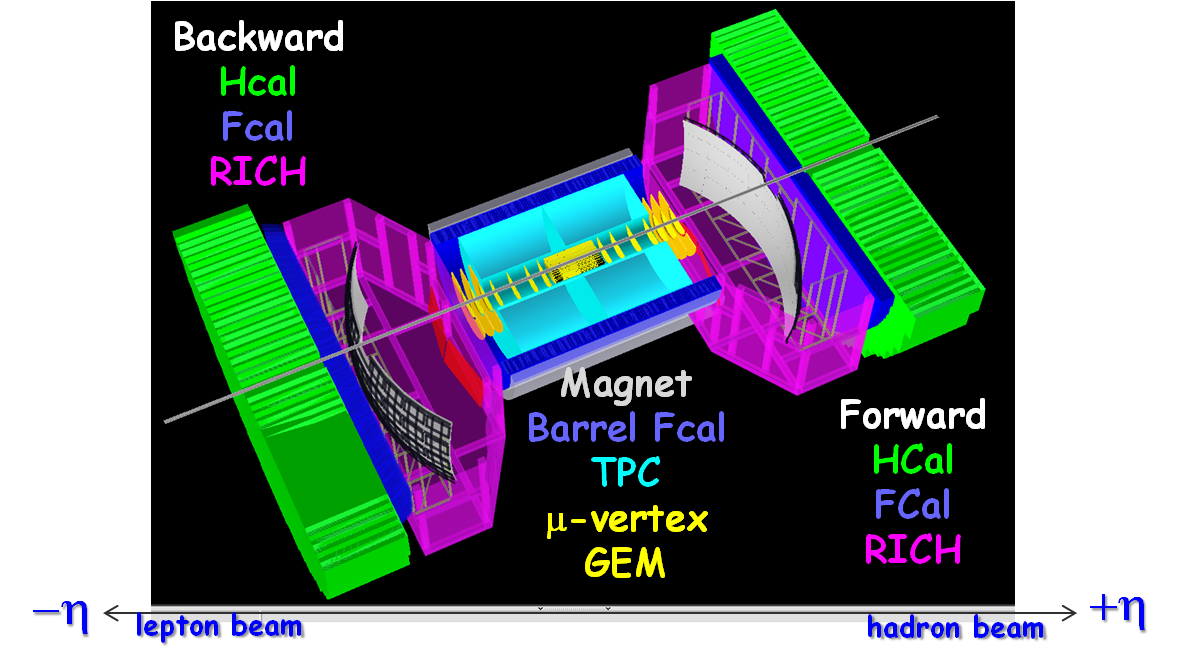
\includegraphics[width=0.9\textwidth]{plots/chpt4/eRHIC_model_detector.png}
\caption[eRHIC detector design]{
Schematics view of the model detector design for eRHIC. The plot is from BNL eRHIC study group.}
\label{fig:detector_eRHIC}
\end{figure}

This eRHIC model detector dedicated to EIC physics is consisted of several major parts.


\begin{itemize}
\item Tracking detectors. The tracking system of the baseline eRHIC detector
will consist of a time projection chamber (TPC), gas electron multiplier (GEM)
and silicon trackers spanning a range $-4<\eta<4$, shown in
Fig.~\ref{fig:tracking_eRHIC}. It is very important to have excellent momentum
resolution over a wide-rapidity range. 
\begin{itemize}
\item Backward/Forward Silicon Tracker: $2<|\eta|<4$, designed with 5-7 MAPS 
(Monolithic Active Sensor Pixels) technology discs.

\item Backward/Forward GEM Tracker: $1.5<|\eta|<3$, designed with 2-3 GEM tracker discs.

\item TPC: $|\eta|<1.5$, deliver hits for pseudorapidity up to $|\eta|\sim2$, but the
range with sufficient number of hits is indicated as above. 

\item Vertex Silicon Tracker: $|\eta|<1$, to be equipped with 4-6 layers of MAPS silicon sensors
similar to the STAR HFT or ALICE ITS upgrade.

\end{itemize}

\end{itemize}


\begin{itemize}
\item Electromagnetic Calorimeter (ECal). The end-cap and barrel regions of
the detector will be equipped with electromagnetic calorimeters covering
$-4<\eta<4$. The different electromagnetic calorimeters have different technologies to account for the different requirements. 


\begin{itemize}
\item Forward ECal: $1<\eta<4$, the requirements for the forward ECal are relatively
moderate as its main function is to detect leptons from the decay of VMs and
photons from dominately $\pi^{0}$ decay. Currently the idea is to have a scintillating fiber tungsten
powder sampling calorimeter. 
\item Barrel ECal: $-1<\eta<1$, this calorimeter needs to provide PID for the scattered lepton at high $Q^{2}$ and leptons from VM-decays, the energy of these leptons will be determined from the tracking detectors. 
The same technology as the forward ECal has been considered for the barrel ECal.
\item Backward ECal: $-4<\eta<-1$, this calorimeter needs to provide PID for the scattered
lepton. It is especially important for the scattered lepton at low $Q^{2}$. At
higher center-of-mass energies photons from $\pi^{0}$ decays, the DVCS and BH
process are in the acceptance of the backward ECal. Since the requirements in
energy and angular resolution are most demanding, it is advised to have a PWO
crystal calorimeter
\end{itemize}
\end{itemize}

\begin{itemize}
\item Hadron Calorimeter (HCal). The resolution requirements for HCal are relatively moderate, therefore standard HCal techniques are totally applicable.  

\begin{itemize}

\item Forward HCal: $1<\eta<4$, this HCal is mainly for jet physics in DIS and diffractive events. It helps define a clean rapidity gap.

\item Backward HCal: $-4<\eta<-1$, this HCal is designed for the jet physics and will be useful to identify scattered lepton at low $Q^{2}$
when ECal is not enough to separate leptons from hadrons. 

\end{itemize}
\end{itemize}

\begin{figure}
\centering
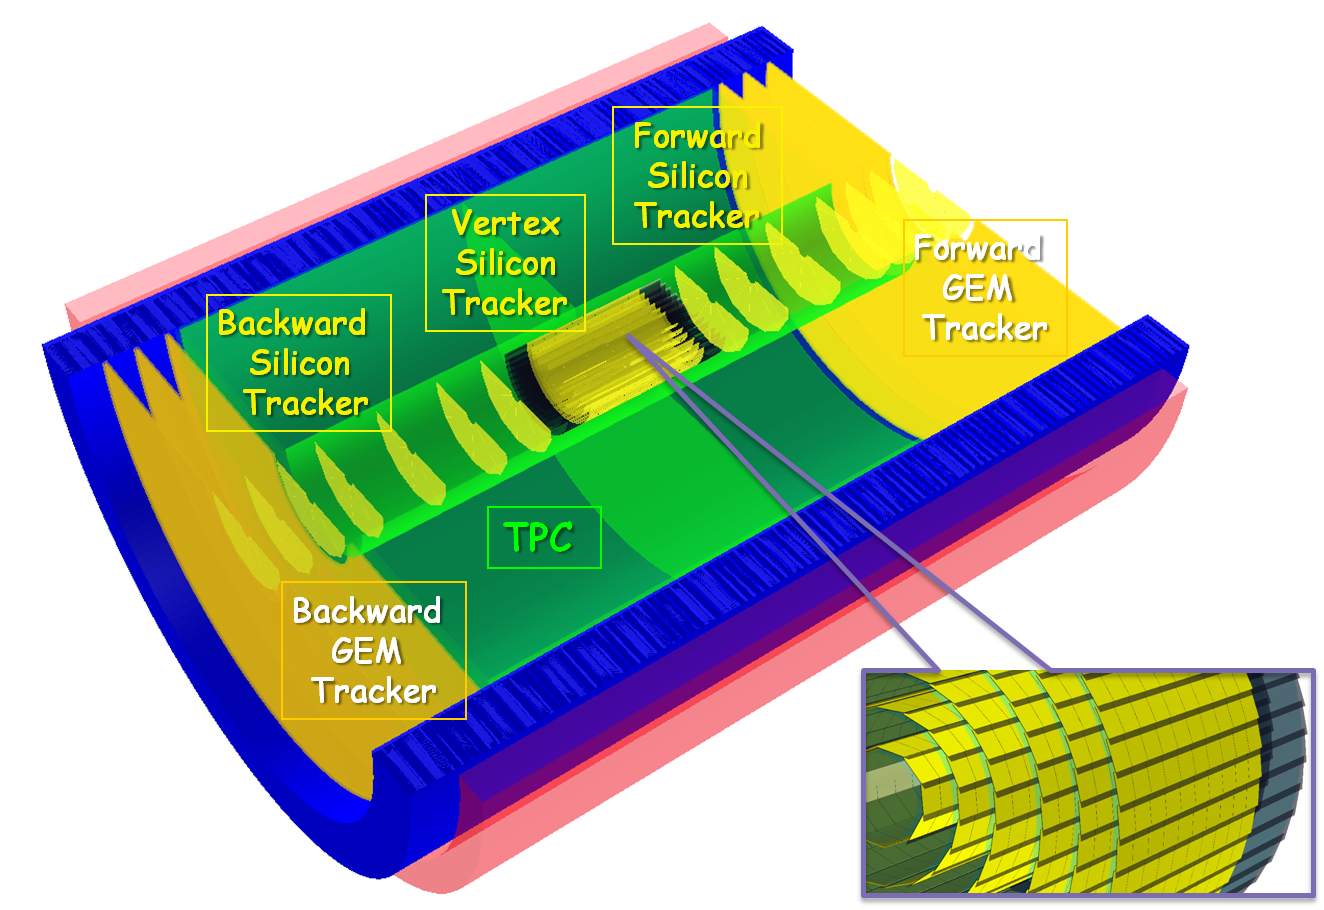
\includegraphics[width=0.9\textwidth]{plots/chpt4/eRHIC_model_tracking.png}
\caption[Tracking system of the eRHIC model detector design]{
Schematic view of the tracking system used in the model detector design for eRHIC. The plot is from BNL eRHIC study group.}
\label{fig:tracking_eRHIC}
\end{figure}


Particle identification for different purpose relies on different combinational
method. $\pi, K, p$ separation can be achieved in central rapidity region
$\eta<1$ with DIRC or proximity focusing Aerogel-RICH plus the $dE/dx$ from TPC
energy loss. The separation in $1<|\eta|<3$ is obtained in RICH, where a very
good meomentum resolution from the tracking is needed.

Lepton identification mainly relies on the $E/p$ in the region $-3<\eta<3$. For
$1<|\eta|<3$, additional HCal response and $\gamma$ suppression via tracking can
be applied to find electrons. In $|\eta|>3$, combinational ECal and HCal
responses and $\gamma$ suppression via tracking will provide a clean access to
the scattered lepton.


\subsection{eSTAR and ePHENIX}
Other than the model detector design which is dedicated to the DIS physics, it
is also possible to evolve the current STAR and PHENIX experimental facility to
eSTAR and ePHENIX~\cite{Adare:2014aaa} in the future with some upgrades. 


\begin{figure}
\centering
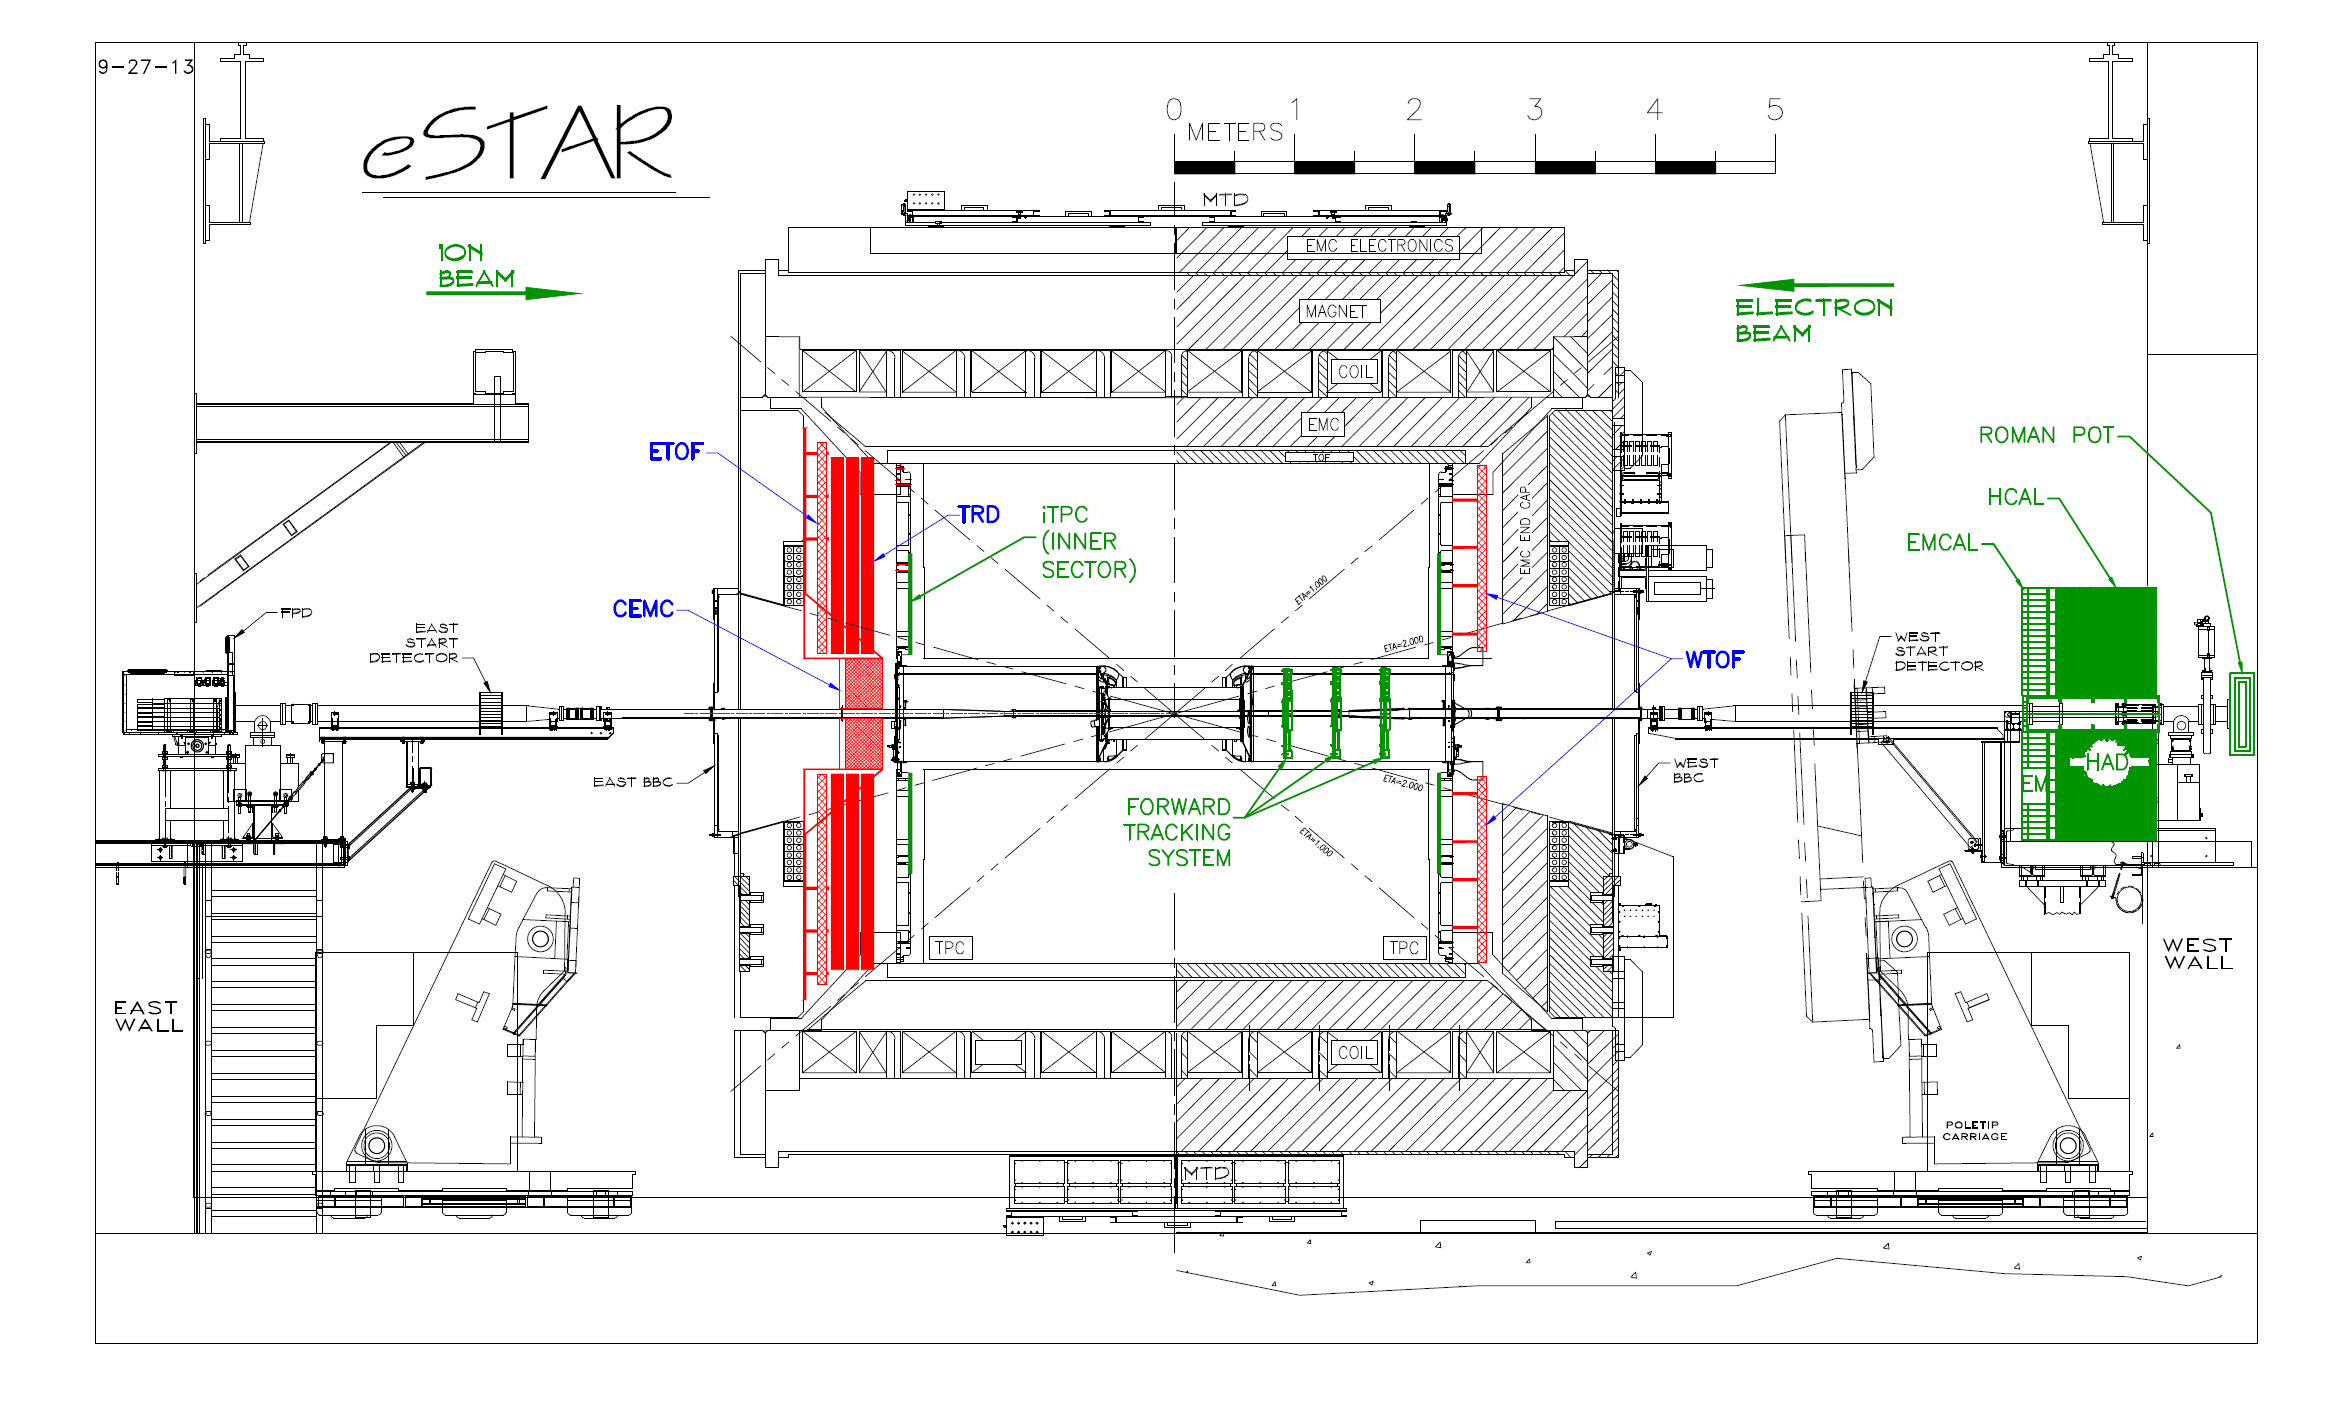
\includegraphics[width=0.8\textwidth]{plots/chpt4/eSTAR_layout.png}
\caption[Layout of eSTAR detector concept]{
eSTAR layout with proposed upgrades. Electron beam is from right to left while hadron beam is from let to right. The plot is Ref.~\cite{star_LoI}.}
\label{fig:eSTAR_layout}
\end{figure}

The proposed eSTAR detector configuration has been shown in
Fig.~\ref{fig:eSTAR_layout}. To identify the scattered lepton in $|\eta|>1$,
endcap TOF on both sides covering $1<|\eta|<2$ and GEM based TRD covering
$-2<\eta<-1$ will be added. Also, before the completion of RHIC program, a
forward tracking system with associated forward calorimeters will be installed.

The ePHENIX detector is going to reuse the superconducting solenoid and the
calorimeter system of sPHENIX, the proposed upgrade of PHENIX focusing on jet
physics. A possible layout has been shown in Fig.~\ref{fig:ePhenix_layout}.
Other than the reusable subsystems from sPHENIX, a few more new subsystems will
be added to the ePHENIX detector. The GEM detectors are needed in both electron
and hadron going direction, providing tracking information for the region
$|\eta|>1$. Endcap electromagnetic calorimeters will be equipped to have full
coverage over $-4<\eta<4$.
\begin{figure}
\centering
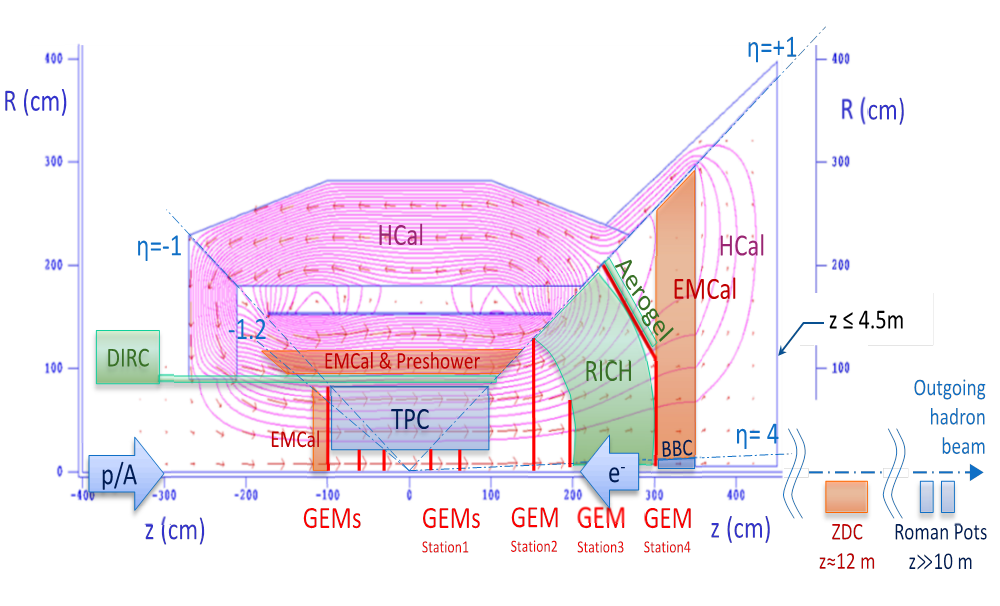
\includegraphics[width=0.8\textwidth]{plots/chpt4/ePhenix_layout.png}
\caption[Layout of ePHENIX detector concept]{
A cross view of the ePHENIX detector concept. The plot is Ref.~\cite{Adare:2014aaa}.}
\label{fig:ePhenix_layout}
\end{figure}

